\chapter{Convection}
Convective heat transfer is the study of heat transport processes due to the flow of fluids \cite{Bejan2013}. Inside a fluid there may be different temperatures: some parts of it can have a higher temperature and others a lower temperature. The movement of liquids or gases combined with the temperature gradient causes convection \cite{Bergman2011}.

This heat transfer occurs in the layers of a fluid, or can also occur between a solid and the fluid that is in contact with it. In both cases, the heat transfer depends on the properties of the fluid and its motion. As a consequence, to understand the heat transfer in a fluid or between a solid and a fluid, it is necessary to know the properties of the fluid itself.

\section{The generic convection-diffusion equation}
The motion of a fluid is described by the Navier-Stokes equations or conservation equations. As discussed in section \ref{ConservationEquations}, the Navier-Stokes equations are a particular case of the generic convection diffusion-equation \ref{GCDE}:
\begin{equation}
\frac{\partial}{\partial t}\left(\rho\phi\right)+\nabla\cdot\left(\rho\vec{v}\phi\right)=\nabla\cdot\left(\Gamma\nabla\phi\right)+S_{phi}
\label{GCDE}
\end{equation}
where $\rho$ is the density, $\vec{v}$ the velocity, $\Gamma$ the diffusion coefficient, $S_{\phi}$ the source term, and $\phi$ the general variable that is going to be studied. Some examples can be found in table \ref{convdifeq}.

\section{Discretization}
\label{DiscretizationSH}
It is necessary to discretize equation \ref{GCDE} in space and time. The spatial discretization is done dividing the domain in different control volumes with a Cartesian grid. The node centred distribution is used, as specified in figure \ref{SHmesh}. The boundary nodes are in blue and the inner nodes in black.
\begin{figure}
	\centering
	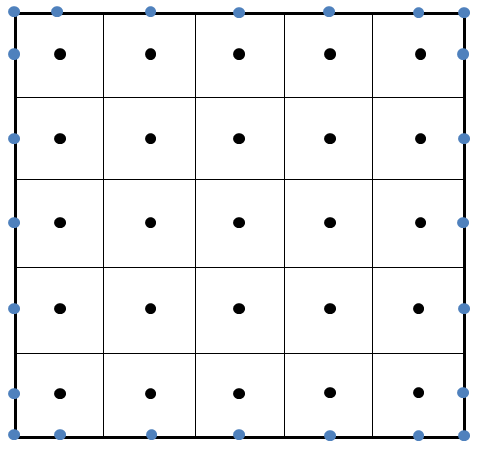
\includegraphics[scale=0.6]{SmithHutton/mesh}
	\caption{Mesh of the Smith-Hutton problem}
	\label{SHmesh}
\end{figure}

To do so, it is easier to start with the discretization of the mass equation \ref{massequation}:
\begin{equation}
\frac{\partial\rho}{\partial t}+\nabla\cdot\left(\rho\vec{v}\right)=0
\label{massequation}
\end{equation}
The first step is to integrate Equation \ref{massequation} over time and space. Taking only the first term of the equation:
\begin{multline}
\int_{t^{n}}^{t^{n+1}}\int_{V_{P}}^{}\frac{\partial\rho}{\partial t}dVdt=\int_{t^{n}}^{t^{n+1}}V_{P}\frac{\partial\bar{\rho}_{P}}{\partial t}dt=V_{P}\left(\bar{\rho}_{P}^{n+1}-\bar{\rho}_{P}^{n}\right)\approx \\
V_{P}\left(\rho_{P}^{n+1}-\rho_{P}^{n}\right)=V_{P}\left(\rho_{P}-\rho_{0}\right)
\end{multline}
Using the Divergence Theorem, the second term of the mass equation transforms into a surface integral. Then, to integrate over time, an implicit scheme is used.
\begin{multline}
\int_{t^{n}}^{t^{n+1}}\int_{V_{P}}^{}\nabla\cdot\left(\rho\vec{v}\right)dVdt=\int_{t^{n}}^{t^{n+1}}\int_{S_{f}}^{}\rho\vec{v}\cdot\vec{n}dSdt= \\
\int_{t^{n}}^{t^{n+1}}\left(\dot{m}_{e}-dot{m}_{w}+dot{m}_{n}-dot{m}_{s}\right)dt\approx\left[\dot{m}_{e}-dot{m}_{w}+dot{m}_{n}-dot{m}_{s}\right]^{n+1}\Delta t
\end{multline}
The final discretized mass equation is \ref{Discretizedmasseq2D}:
\begin{equation}
\frac{V_{P}\left(\rho_{P}-\rho_{0}\right)}{\Delta t}+\dot{m}_{e}-dot{m}_{w}+dot{m}_{n}-dot{m}_{s}=0
\label{Discretizedmasseq2D}
\end{equation}
The discretization of the convection-diffusion equation is very similar to that of the mass equation. Integrating over the volume the transport term of equation \ref{GCDE} and applying the Divergence Theorem:
\begin{equation}
\int_{V_{P}}\nabla\cdot\left(\rho\vec{v}\phi\right)=\int_{S_{f}}\rho\phi\vec{v}\cdot\vec{n}dS=\dot{m}_{e}\phi_{e}-\dot{m}_{w}\phi_{w}+\dot{m}_{n}\phi_{n}-\dot{m}_{s}\phi_{s}
\end{equation}
The same procedure is used for the diffusion term of equation \ref{GCDE}:
\begin{multline}
\int_{V_{P}}\nabla\cdot\left(\Gamma\nabla\phi\right)=\int_{S_{f}}\Gamma\cdot\nabla\phi\cdot\vec{n}dS=-\Gamma_{w}\frac{\partial\phi}{\partial x}\big|_{w}S_{w}+\Gamma_{e}\frac{\partial\phi}{\partial x}\big|_{e}S_{e}-\Gamma_{s}\frac{\partial\phi}{\partial x}\big|_{s}S_{s}+\Gamma_{n}\frac{\partial\phi}{\partial x}\big|_{n}S_{n}\approx \\
D_{e}\left(\phi_{E}-\phi_{P}\right)-D_{w}\left(\phi_{P}-\phi_{W}\right)+D_{n}\left(\phi_{N}-\phi_{P}\right)-D_{s}\left(\phi_{P}-\phi_{S}\right)\big|
\end{multline}
where
\begin{equation}
D_{e}=\frac{\Gamma_{e}S_{e}}{d_{PE}}
\end{equation}
\begin{equation}
D_{w}=\frac{\Gamma_{w}S_{w}}{d_{PW}}
\end{equation}
\begin{equation}
D_{n}=\frac{\Gamma_{n}S_{n}}{d_{PN}}
\end{equation}
\begin{equation}
D_{s}=\frac{\Gamma_{s}S_{s}}{d_{PS}}
\end{equation}
To simplify the source term, it is linearized:
\begin{equation}
\int_{V_{P}}S_{\phi}dV\approx S_{\phi,P}V_{P}=\left(S_{c}^{\phi}+S_{p}^{\phi}\phi_{P}\right)V_{P}
\end{equation}
So that the resulting discretized equation is:
\begin{multline}
\frac{\rho_{P}\phi_{P}-\rho_{P}^{0}\phi_{P}^{0}}{\Delta t}V_{P}+\dot{m}_{e}\phi_{e}-\dot{m}_{w}\phi_{w}+\dot{m}_{n}\phi_{n}-\dot{m}_{s}\phi_{s}= \\
D_{e}\left(\phi_{E}-\phi_{P}\right)-D_{w}\left(\phi_{P}-\phi_{W}\right)+D_{n}\left(\phi_{N}-\phi_{P}\right)-D_{s}\left(\phi_{P}-\phi_{S}\right)+S_{\phi,P}V_{P}
\label{IntermGCDE}
\end{multline}
Multiplying by $\phi$ the discretized mass equation \ref{Discretizedmasseq2D} and subtracting the result in \ref{IntermGCDE}, the discretized convection-diffusion equation is obtained:
\begin{multline}
\rho_{P}^{0}\frac{\phi_{P}-\phi_{P}^{0}}{\Delta t}V_{P}+\dot{m}_{e}\left(\phi_{e}-\phi_{P}\right)-\dot{m}_{w}\left(\phi_{w}-\phi_{P}\right)+\dot{m}_{n}\left(\phi_{n}-\phi_{P}\right)-\dot{m}_{s}\left(\phi_{s}-\phi_{P}\right)= \\
D_{e}\left(\phi_{E}-\phi_{P}\right)-D_{w}\left(\phi_{P}-\phi_{W}\right)+D_{n}\left(\phi_{N}-\phi_{P}\right)-D_{s}\left(\phi_{P}-\phi_{S}\right)+S_{\phi,P}V_{P}
\label{DiscretizedGCDE}
\end{multline}
The final step is to find an expression to evaluate the properties in the faces of the control volume, not in the nodes.

\section{Evaluation of the value in the faces}
To simplify the problem, a new variable is introduced to the problem: the total flux \cite{Patankar1980}. This variable is split in the two dimensions of the problem, the flux in the x-direction and the flux in the y-direction.
\begin{equation}
J_{x}\equiv\rho u\phi-\Gamma\frac{\partial\phi}{\partial x}
\label{fluxx}
\end{equation}
\begin{equation}
J_{y}\equiv\rho v\phi-\Gamma\frac{\partial\phi}{\partial y}
\label{fluxy}
\end{equation}
Introducing the expressions of the total flux \ref{fluxx} and \ref{fluxy} to equation \ref{DiscretizedGCDE}, the discretized convection diffusion equation becomes:
\begin{multline}
\rho_{P}^{0}\frac{\phi_{P}-\phi_{P}^{0}}{\Delta t}V_{P}+\left(J_{e}-F_{e}\phi_{P}\right)-\left(J_{w}-F_{w}\phi_{P}\right)+\left(J_{n}-F_{n}\phi_{P}\right)-\left(J_{s}-F_{s}\phi_{P}\right)= \\
\left(S_{p}^{\phi}\phi_{P}\right)V_{P}
\label{FinalDiscrGCDE}
\end{multline}
where the flow rates are:
\begin{equation}
F_{e}=\left(\rho u\right)_{e}S_{e}
\end{equation}
\begin{equation}
F_{w}=\left(\rho u\right)_{w}S_{w}
\end{equation}
\begin{equation}
F_{n}=\left(\rho v\right)_{n}S_{n}
\end{equation}
\begin{equation}
F_{s}=\left(\rho v\right)_{s}S_{s}
\end{equation}
However, it is necessary to know how the fluxes are going to be evaluated. In order to use non-dimensional numbers, a new variable is defined:
\begin{equation}
J^{*}\equiv\frac{J\delta}{\Gamma}=P\phi-\frac{d\phi}{d\left(x/\delta\right)}
\end{equation}
where $P$ is the Péclet number and $\delta$ is the distance between the point that is going to be studied $i$, and the point next to it, $i+1$. The value of $\phi$ and the value of the gradient $d\phi/d\left(x/\delta\right)$ are a combination of the $\phi_{i}$ and $\phi_{i+1}$, so that $J^{*}$ can be expressed as \cite{Patankar1980}:
\begin{equation}
J^{*}=B\phi_{i}-A\phi_{i+1}
\end{equation}
The coefficients $A$ and $B$ are dimensionless and depend on the Péclet number. However, $B$ is a combination of $A$ and the Péclet number, and both coefficients are symmetric \cite{Patankar1980}. Taking these properties into account and introducing the operator $\textlbrackdbl A,B\textrbrackdbl$ that denotes the greater of $A$ and $B$, it can be deduced that:
\begin{equation}
A\left(P\right)=A\left(|P|\right)+\textlbrackdbl-P,0\textrbrackdbl
\label{A}
\end{equation}
\begin{equation}
B\left(P\right)=A\left(|P|\right)+\textlbrackdbl-P,0\textrbrackdbl
\label{B}
\end{equation}
Introducing equations \ref{A} and \ref{B} into \ref{FinalDiscrGCDE}, the following formulation is obtained:
\begin{equation}
a_{P}\phi_{P}=a_{E}\phi_{E}+a_{W}\phi_{W}+a_{N}\phi_{N}+a_{S}\phi_{S}+b_{P}
\label{DiscretizedEquGCDE}
\end{equation}
where
\begin{equation}
a_{E}=D_{e}A\left(|P_{e}|\right)+\textlbrackdbl-F_{e},0\textrbrackdbl
\end{equation}
\begin{equation}
a_{W}=D_{w}A\left(|P_{w}|\right)+\textlbrackdbl F_{w},0\textrbrackdbl
\end{equation}
\begin{equation}
a_{N}=D_{n}A\left(|P_{n}|\right)+\textlbrackdbl-F_{n},0\textrbrackdbl
\end{equation}
\begin{equation}
a_{S}=D_{s}A\left(|P_{s}|\right)+\textlbrackdbl-F_{s},0\textrbrackdbl
\end{equation}
\begin{equation}
a_{P}=a_{E}+a_{W}+a_{N}+a_{S}+\frac{\rho_{P}^{0}V_{P}}{\Delta t}-S_{P}V_{P}
\end{equation}
\begin{equation}
b_{P}=S_{c}V_{P}+\frac{\rho_{P}^{0}V_{P}}{\Delta t}\phi_{P}^{0}
\end{equation}
And the Péclet numbers are:
\begin{equation}
P_{e}=\frac{F_{e}}{D_{e}}
\end{equation}
\begin{equation}
P_{w}=\frac{F_{w}}{D_{w}}
\end{equation}
\begin{equation}
P_{n}=\frac{F_{n}}{D_{n}}
\end{equation}
\begin{equation}
P_{s}=\frac{F_{s}}{D_{s}}
\end{equation}
The only operation that should be defined is the value of the coefficient $A$. This value depends on the integration scheme that is going to be used. Some of its values are listed in table \ref{Patankarvalues}.
\begin{table}[h]
	\centering
	\begin{tabular}{ |c|c| }
		\hline
		Scheme & Formula for $A\left(|P_{s}|\right)$ \\ \hline
		Central difference (CDS) & $1-0.5|P|$ \\ \hline
		Upwind (UDS) & $1$ \\ \hline
		Hybrid (HDS) & $\textlbrackdbl0,1-0.5|P|\textrbrackdbl$ \\ \hline
		Power law (PLDS) & $\textlbrackdbl0,\left(1-0.5|P|\right)^{5}\textrbrackdbl$ \\ \hline
		Exponential (EDS) & $|P|/\left[exp\left(|P|\right)-1\right]$ \\ \hline
	\end{tabular}
	\caption{Function $A(|P|)$ for different schemes\cite{Patankar1980}}
	\label{Patankarvalues}
\end{table}